\chapter{Analysis and Design Approach} \label{chapter:analysis_and_design}
\section{Previous Architecture}
The figure below illustrates the previous architecture of the ASR system, which was deployed on a Kubernetes cluster hosted on AWS.

\begin{figure}[!ht]
    \centering
    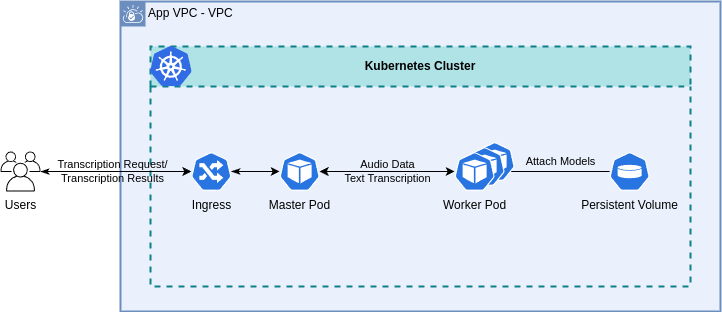
\includegraphics[width=\textwidth]{figures/previous_architecture.drawio.png}
    \caption{Previous Architecture of the ASR System}
\end{figure}

In the previous architecture, transcription requests were routed through an NGINX Ingress Controller. The Ingress Controller forwarded these requests to the master pod, which acted as the main server responsible for handling transcription tasks. Upon receiving a request, the master pod authenticated it and, if a worker pod was available, initiated a WebSocket connection to the worker pod. The audio data was then transmitted to the worker pod for transcription.

Each worker pod was associated with a model attached via a Persistent Volume Claim (PVC). After processing the audio data, the worker pod sent the transcription results back to the master pod, which subsequently forwarded them to the client.

\subsection{Limitation 1: Tight Coupling}
The previous architecture was the tight coupling between the master and worker pods due to the synchronous communication via the WebSocket connection. If the master pod crashed, the WebSocket connection would be lost, interrupting the transcription process. Similarly, if a worker pod failed, any ongoing transcription tasks would be lost. This synchronous design hindered fault tolerance and scalability, as the components were highly dependent on one another for successful operation.

\subsubsection{Proposed Solution}
To address the limitation, the new architecture, illustrated in Figure \ref{fig:decouple}, introduces a decoupled design using RabbitMQ as a message queue.

\begin{figure}[!ht]
    \centering
    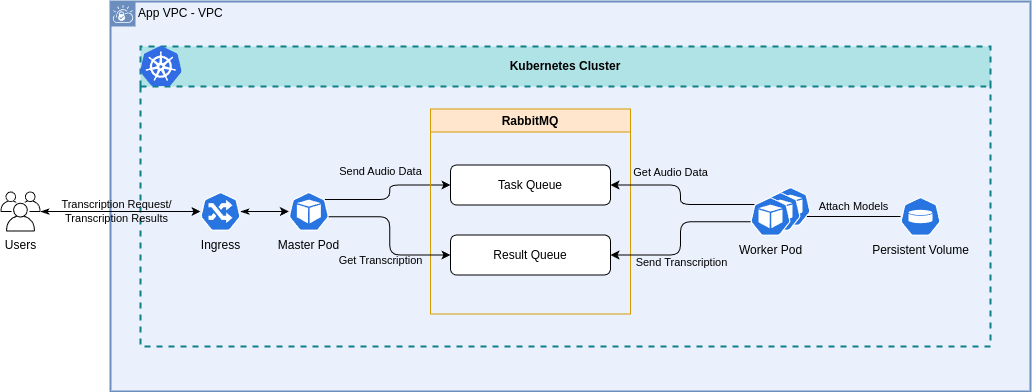
\includegraphics[width=\textwidth]{figures/decouple.drawio.png}
    \caption{Decoupling the Master and Worker Pods}
    \label{fig:decouple}
\end{figure}

In the new architecture, the master pod sends audio data to a task message queue (RabbitMQ). Worker pods consume the audio data from this queue, process it, and send the transcription results to a results message queue. The master pod retrieves the transcription results from the results message queue and sends them back to the client.

This decoupled, asynchronous communication model eliminates the tight coupling between the master and worker pods. It allows each component to scale independently, improving both scalability and fault tolerance.

\subsection{Limitation 2: Stateful Components}
Another contraint of the previous architecture was that it relied on stateful components within both the master and worker pods. For instance, the worker pod stored audio data in an in-memory queue. If the worker pod crashed, the audio data in the queue would be lost, requiring the client to retransmit the data. This dependency on volatile storage not only complicated fault handling but also further exacerbated the system’s lack of fault tolerance.

\subsubsection{Proposed Solution}
Additionally, the state of the application is now stored in Redis. By persisting the application state in Redis, the system becomes more resilient to crashes. If any service fails, it can retrieve the necessary state information from Redis or the message queues, ensuring minimal disruption and faster recovery.

\subsection{Limitation 3: Scaling}
The previous deployment of the ASR system relied on a single master pod instance. This created a single point of failure—if the master pod crashed, there would be no backup instance to route requests, causing service disruptions.

Additionally, scaling the number of worker pods was a manual process, requiring administrators to manually update the number of replicas. This approach was inefficient and often led to delays in responding to changes in system load, impacting the system’s ability to handle fluctuations in traffic effectively.

\subsubsection{Proposed Solution}
To address these limitations, Kubernetes Horizontal Pod Autoscaler (HPA) was implemented to dynamically scale the number of master pods based on traffic load. This ensures the system can handle increased request volumes during peak times and scale down during off-peak periods, optimizing resource usage and maintaining availability.

For worker pods, a dynamic scaling policy was introduced (See Code \ref{lst:worker_scaling}). This policy adjusts the number of worker pods automatically to meet a predefined \texttt{SCALING\_TARGET}, ensuring that resources are allocated efficiently.



The dynamic scaling policy is managed by an additional service called the Worker Manager, which is described in detail in \hyperref[subsection:worker_manager]{\textit{Chapter 4: Detailed Implementation}}. The Worker Manager monitors the current state of worker pods for each model and adjusts the number of pods accordingly to maintain the scaling target.

Key features of this solution include:
\begin{itemize}
    \item \textbf{Load-based scaling:}  The Worker Manager scales worker pods up or down based on current traffic and processing load, ensuring optimal resource utilization.
    \item \textbf{Minimized scaling disruptions:}  To prevent excessive scaling activity, the scaling policy incorporates a configurable \texttt{CHECK\_INTERVAL} that limits the frequency of scaling operations.
\end{itemize}


\section{Previous Codebase}
In this seciton, we will discuss the limitations of the previous ASR system codebase and propose solutions to address these challenges.

\subsection{Limitation 1: Little to No Documentation}
The previous ASR system codebase lacked sufficient documentation, making it difficult to understand the overall structure and functionality of the system. This lack of clarity posed significant challenges for onboarding new developers, who often had to rely on existing team members for guidance, leading to delays and inefficiencies. Without proper documentation, troubleshooting issues and implementing new features also became time-consuming and error-prone.

\subsubsection{Proposed Solution}
To address these challenges, the new codebase will prioritize comprehensive and clear documentation. A detailed \texttt{README} file will provide an overview of the project, including its architecture, purpose, and key components. Additionally, inline comments will be incorporated throughout the codebase to explain the functionality and intent of each component.

This approach helps to onboard new developers faster, through providing them with more context to understand the system better. Additionally, it ensures maintainability by ensuring the developers can easily understand and modify the codebase in the future.

\subsubsection{Example}
An inline comment explaining the purpose of a function or section of code can significantly improve readability. For instance, Code \ref{lst:code_documentation} shows an example of an inline comment that describes the purpose of a function and its parameters.

\begin{lstlisting}[caption={Example Code Documentation}, label={lst:code_documentation}]
def _start_task(self, task_queue, instance_id=1):
    """
    Start the task and set the state of the worker to BUSY.

    Args:
        task_queue (str): Task queue to be processed by the worker.
        instance_id (int): Instance ID of the task.
    """
\end{lstlisting}

By integrating documentation and inline comments into the development process, the new codebase will improve the maintainability and quick onboarding of new developers.


